\section{关于GAN的创新点的讨论}

在二零二一年八月四日的汇报中, 王老师引用某篇论文对GAN的理解, 其观点为:

\begin{quotation}
    \bfseries
    GAN 中的 Discriminator 可以取代损失函数. 机器学习到深度学习是可以自动学习特征, GAN的出现可以让机器自己学损失函数. 
\end{quotation}  

我对此观点表示怀疑, 这一周中未找到可以支撑此观点的素材. 在此根据我个人想法对该观点进行反驳.

首先, 该观点意味着无需手动设计损失函数, 可用深度模型Discriminator代替, 让机器自己去学习损失函数, 这便意味着, 将任何深度模型的损失函数用Discriminator代替, 应该在学术圈产生和GAN相同爆炸式影响, 现实中并未存在过. 如果存在, 那么在任何领域, 都会有GAN的身影, 之前从未引入GAN的领域 比如图像分类, 也应该有GAN. 通过关键词搜索出论文 ``Self-Supervised GANs With Similarity Loss for Remote Sensing Image Scene Classification'', 很显然从题目就能判断出, 其损失函数为Similarity Loss, 需要自己设计损失函数.

其次, 不需要显示写出损失函数, 那么GAN是无法写出损失函数吗? 在理论层面, GAN的损失函数为:

\begin{equation}
    V = E_{x\sim P_{data}}(logD(x)) + E_{x\sim P_{G}}( log(1-D(x)))
\end{equation}

在实际代码中, 其损失函数的实现为:
\begin{equation}
    V=\frac{1}{m}\sum_{i=1}^{m}logD(x^{i})+\frac{1}{m}log(1-D(\tilde{x}^{i}))
\end{equation}

即GAN的损失函数可以写出, 任何深度学习模型的损失函数都可显示写出. L1, L2, 包括insightface中的arcface, 虽然较为复杂, 但都可以显示写出.

最后, 深度学习的框架为模型, 损失函数, 优化. 模型为函数库, 可表示函数范围, 一般来说, 模型参数越多, 该模型可表示的函数范围越大; 损失函数用来衡量模型训练结果好坏; 优化则是为了在训练中, 找到最优的模型使损失函数值最小. 如果按照观点所示, 可以将深度模型当作损失函数, 那么任何深度模型, 从中截取后半段, 都可当作损失函数. 

总结, 无论从学术的反应, 损失函数是否可写出, 深度学习框架, 该论文的观点显得剑走偏锋, 混淆了深度学习或是机器学习的模型和损失函数部分, 不可取, 根据Ian Fellow在2014年论文中提出观点, GAN的创新点在思想层面是在相互竞争中共同进化; 数学层面上, 通过有限的随机采样, 输入Disciminator来估计$P_{data}$, $P_{G}$的分布差异, 从而得到一个较为强大的Generator可以生成近似$P_{data}$分布的数据. 

% \begin{figure}[!htbp]
%     \centering
%     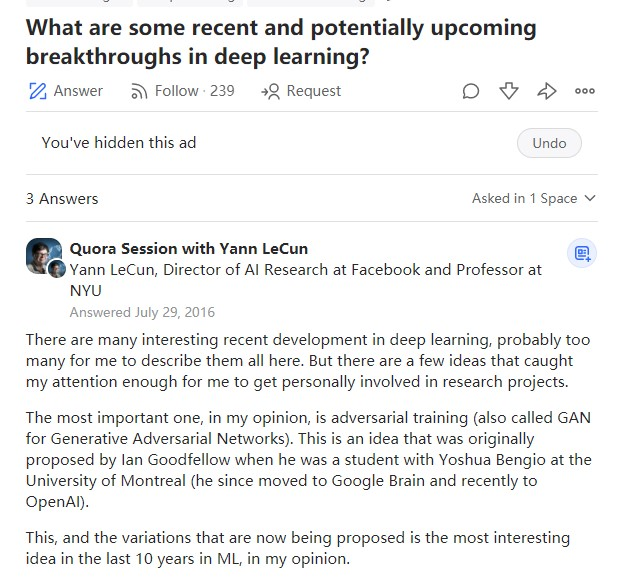
\includegraphics[height=22em]{pic/pic0102.jpg}
%     \caption{Quora 问答}
%     \label{fig:0102}
% \end{figure}

